% Chapter Template

\chapter{The Transmitter} % Main chapter title
\label{Chapter6} 


\section{Introduction}
The transmitter for the sound-based move tracking protocol is in charge of creating the tones representing each centerpiece's current state, and updating those tones each time a centerpiece changes state.

This chapter will detail a proof-of-concept design for a printed circuit board (PCB) containing only nine discrete components capable of generating all the tones required for encoding one centerpiece's state.

This chapter assumes that the reader has a knowledge of basic circuit components like resistors and capacitors.

\section{Requirements}
\label{sec:transmitter-requirements}
This section will detail the constraints within which the transmitter will be required to operate. These constraints include the physical size of the transmitter (Section \ref{subsec:prospects-of-miniaturization}), the precision of tone generation (Section \ref{subsec:precision-of-tone-generation}), the reliability of the transmitter in changing tones to reflect a face turn (Section \ref{subsec:responsiveness-to-face-turns}), and the intensity of output audio that the transmitter can produce (Section \ref{subsec:transmitter-signal-to-noise-ratio}).

\subsection{Prospects of Miniaturization}
\label{subsec:prospects-of-miniaturization}
The transmitter must be both removable and small enough to fit in the center cap of each face of a speedcube.
This requirement stems from two sources.
First, in contrast to all existing smartcubes, most non-smartcubes have small, solid cores (Figure \ref{fig:356-core-closed}) that provide no extra space for the inclusion of any electronics, but do have a small amount of open space within their center cubies (Figure \ref{fig:356-core-open}).
Second, the use of a cube with non-removable, embedded electronics violates the WCA competition regulation 2i \cite{wca-regulations} (See also Section \ref{subsec:competition-regulations}).
\begin{figure}[h]
    \centering
    \caption{Internal pieces of a standard speedcube (Gans 356)}
    \label{fig:356-core}
    \begin{subfigure}{.45\textwidth}
        \centering
        \caption{View of the small, solid plastic core}
        \label{fig:356-core-closed}
        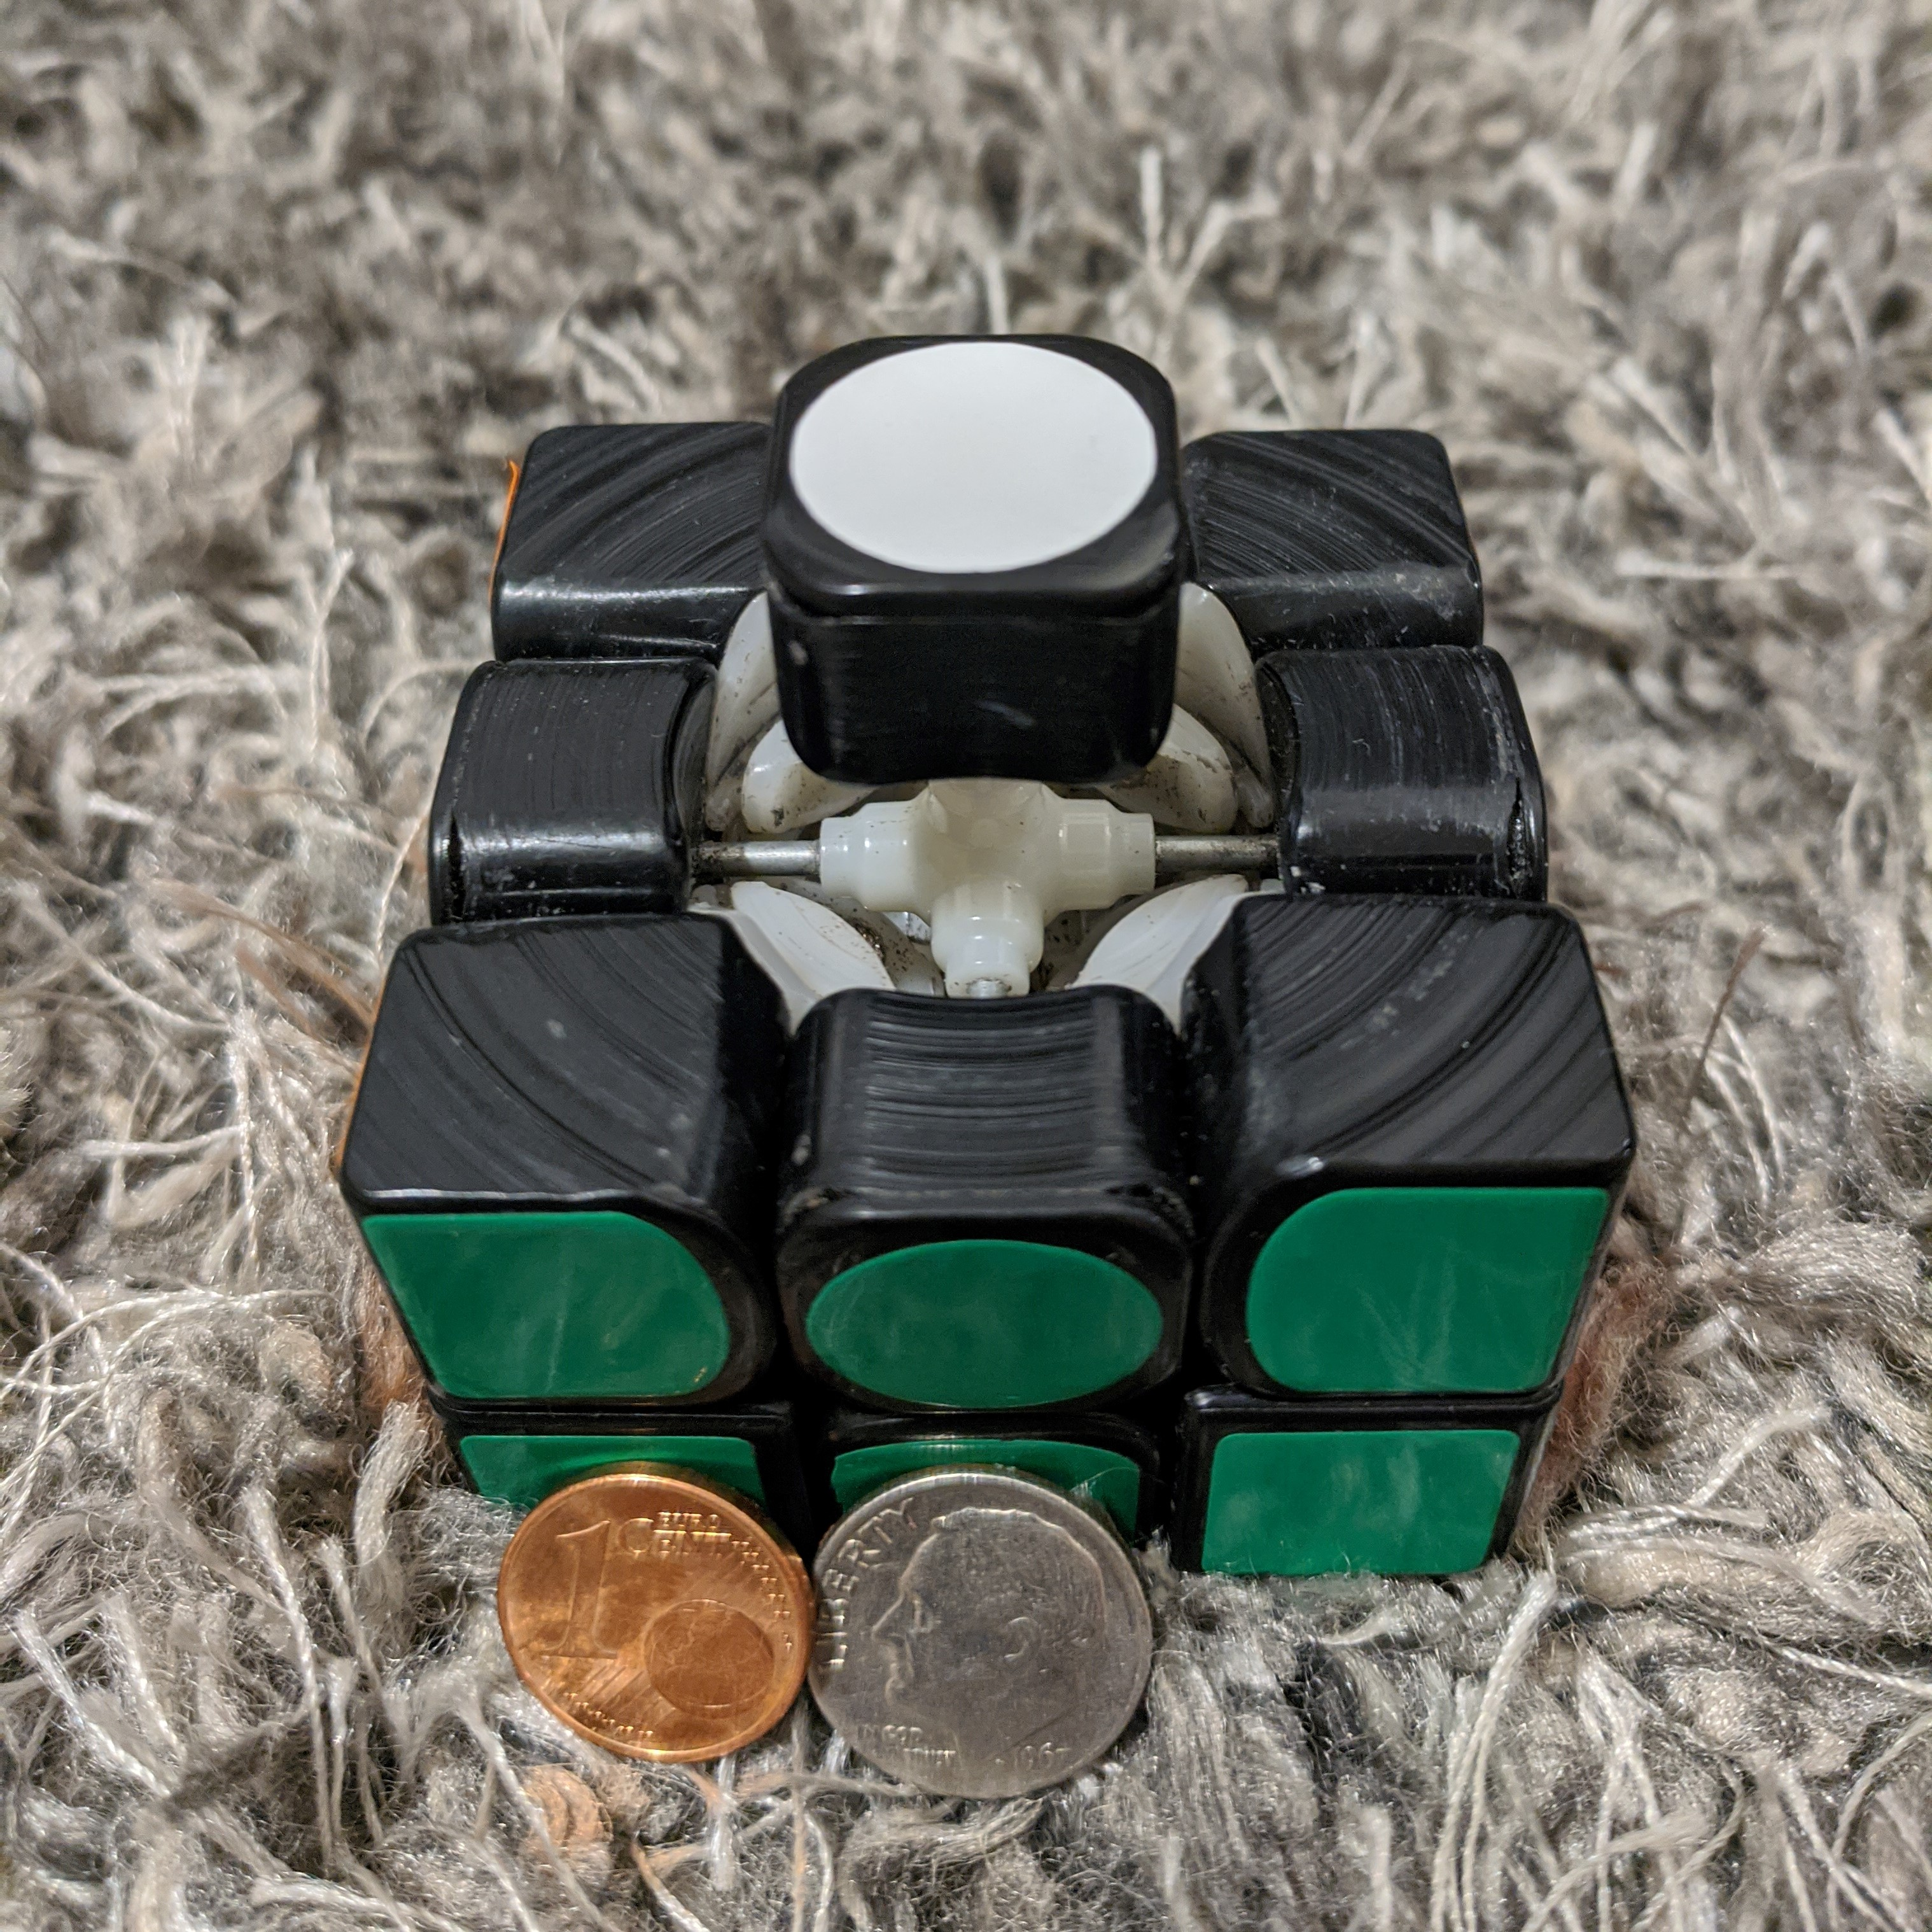
\includegraphics[width=\linewidth]{Figures/6 PCB Design/356_core_cropped.jpg}
    \end{subfigure}
    \begin{subfigure}{.45\textwidth}
        \centering
        \caption{View of the space inside the centerpiece}
        \label{fig:356-core-open}
        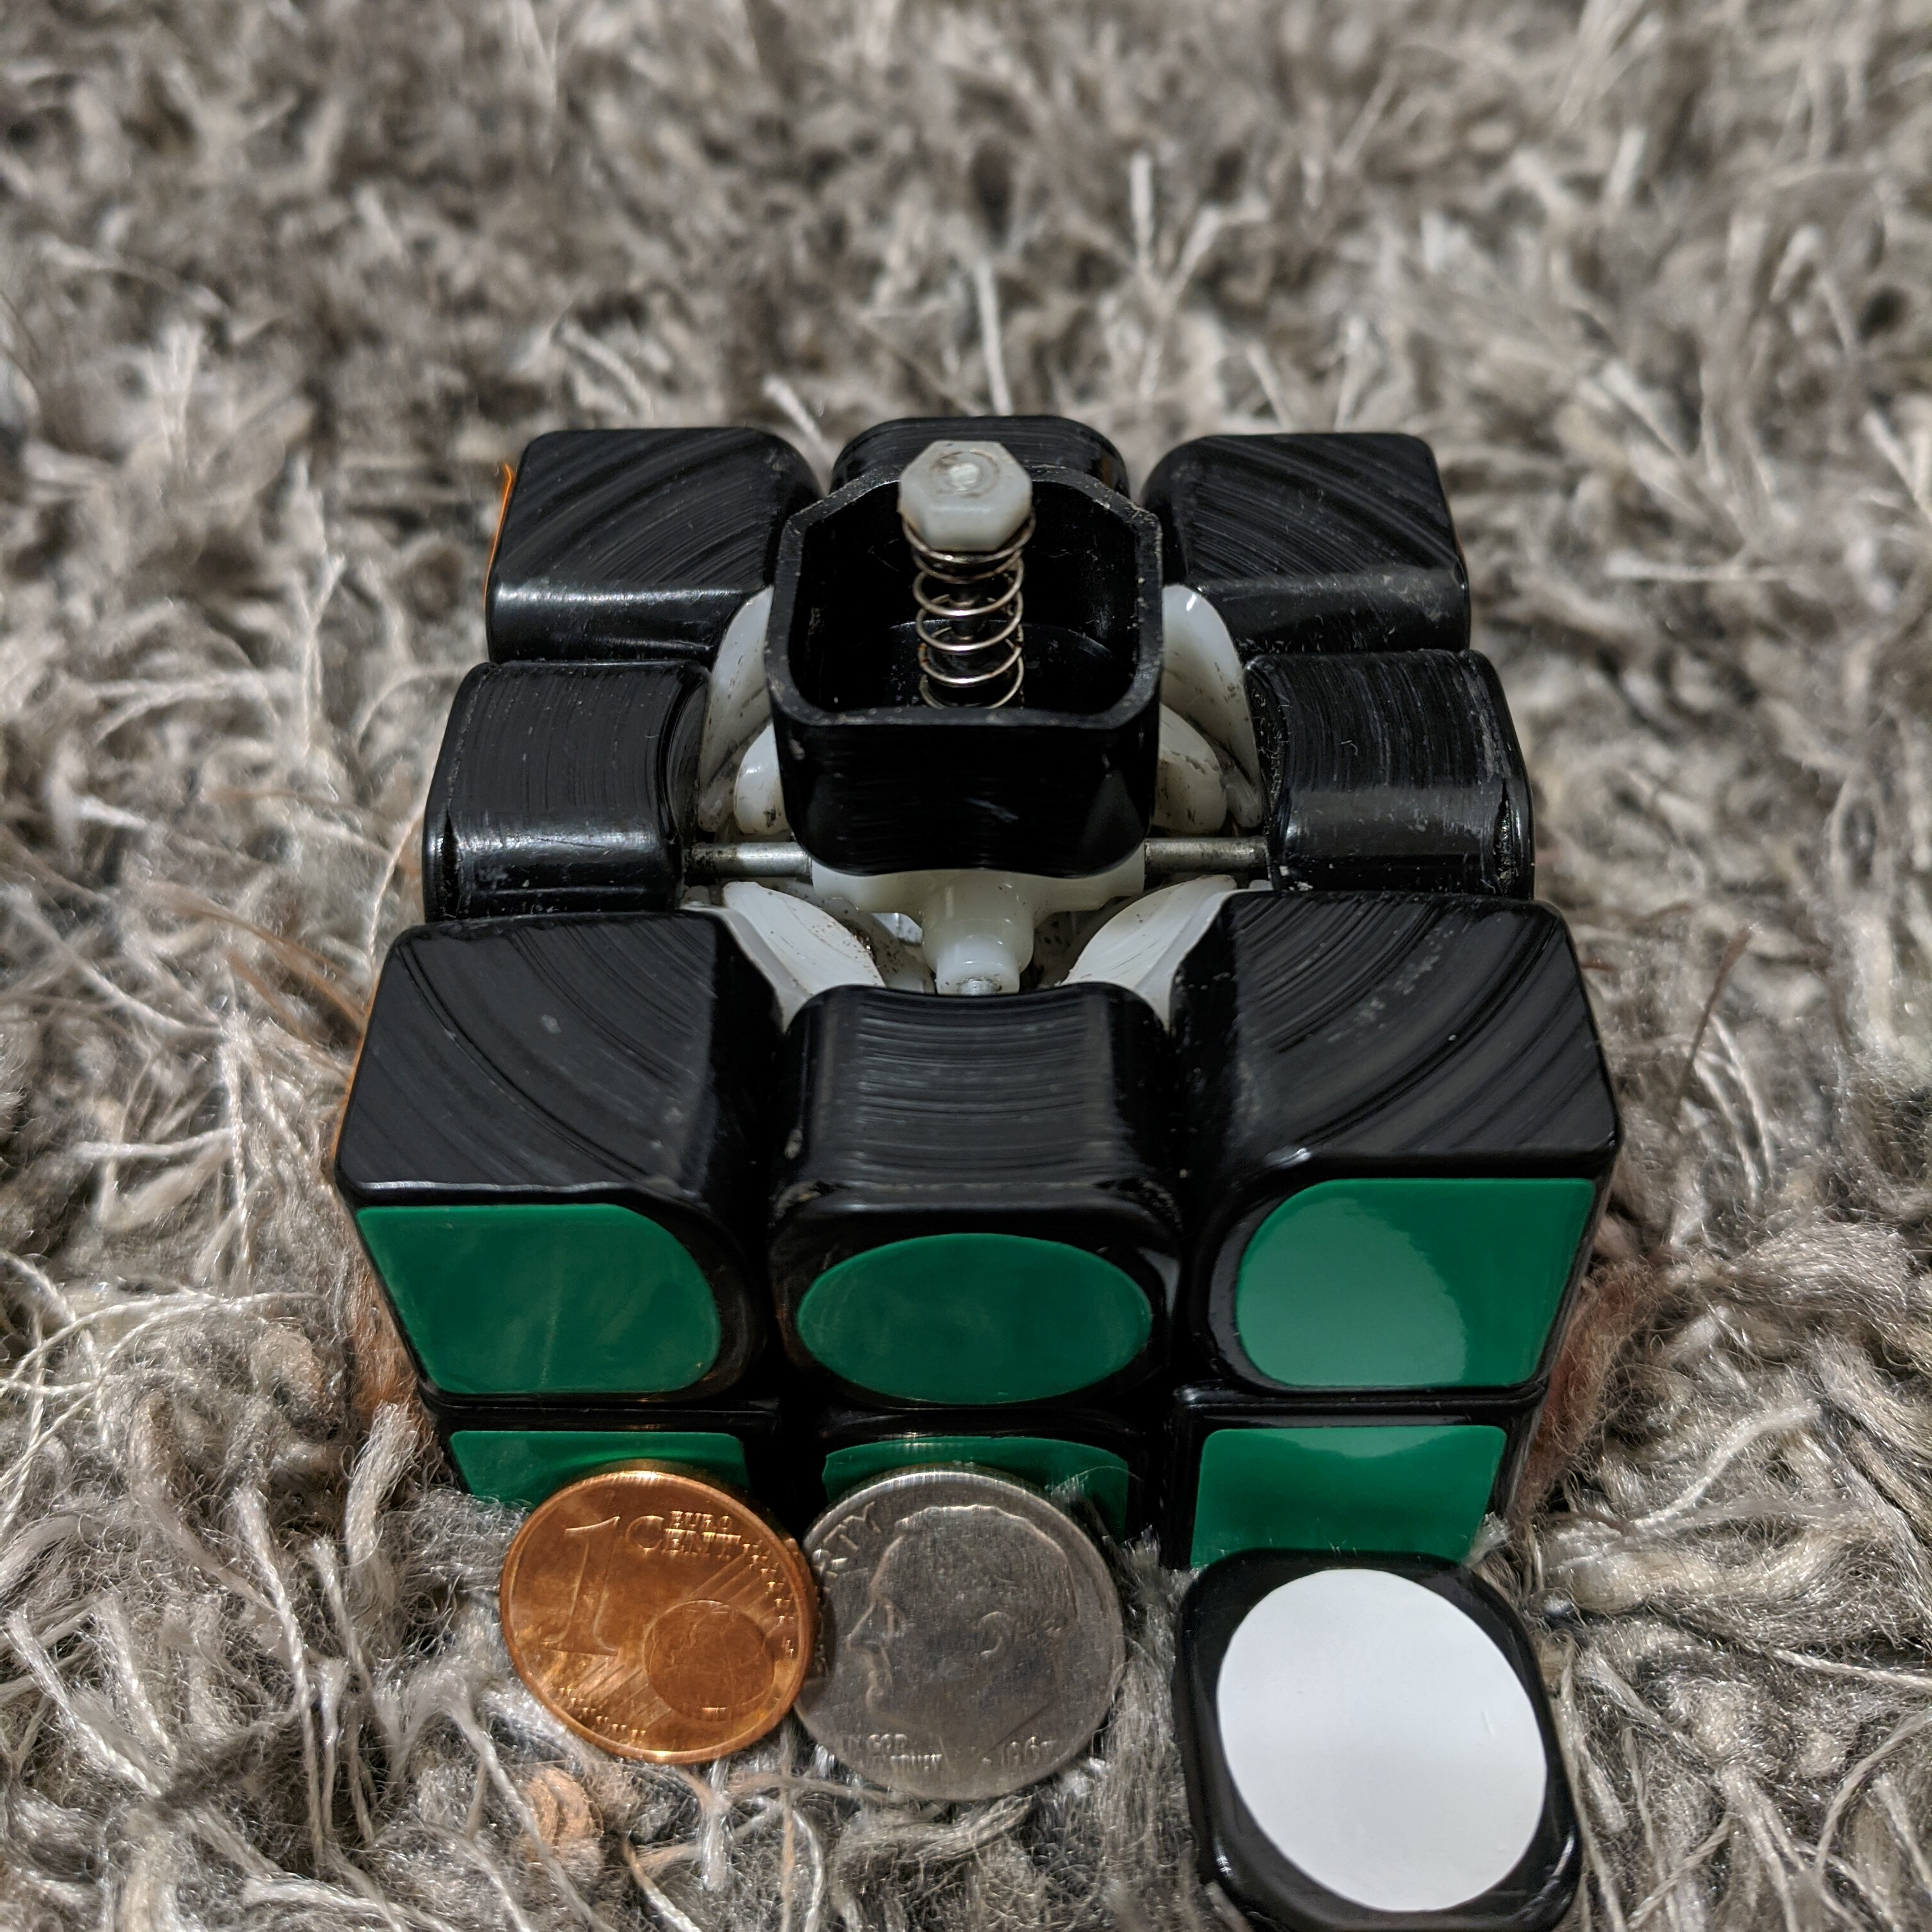
\includegraphics[width=\linewidth]{Figures/6 PCB Design/356_core_open_cropped.jpg}
    \end{subfigure}
\end{figure}

\subsection{Precision of Tone Generation}
\label{subsec:precision-of-tone-generation}
While the receiver specified in Chapter \ref{Chapter5} supports custom state to frequency mappings, it expects that the frequency corresponding to each centerpiece's state stays constant throughout the entire audio recording.
As such, the chosen transmitter design can encode centerpiece states with any frequency (assuming the chosen frequencies work within the constraints specified in Section \ref{sec:protocol-requirements}), but it must produce its chosen frequencies with high precision.

\subsection{Responsiveness to Face Turns}
\label{subsec:responsiveness-to-face-turns}
The chosen transmitter design must respond to an applied face turn by changing the currently transmitted audio frequency to the frequency corresponding to the new centerpiece state.

\subsection{Signal-to-Noise Ratio}
\label{subsec:transmitter-signal-to-noise-ratio}
The transmitter must create tones loud enough to be easily distinguished from ambient noise, including the sound of the Rubik's Cube's own turns.
In light of the above requirement for the transmitter to fit within a center cubie (\ref{subsec:prospects-of-miniaturization}), this requirement will also require the transmitter design to consider how to overcome any audio dampening caused by such an enclosure.


\section{Design}
\label{sec:transmitter-design}
Given the above constrains, this section will detail a design for a printed circuit board capable of precisely generating four distinct tones.

\subsection{The 555 Timer}
\label{sec:the-555-timer}
The core component in this PCB design is a 555 timer, which is a computer chip that facilitates the generation of many types of voltage frequencies in a circuit.

For this transmitter, the 555 timer will be configured to output a square wave voltage signal with a 50\% duty cycle (i.e. "Astable Operation") \cite{icm7555}.
This means the voltage on the output pin will alternate between low and high, spending equal amounts of time in each state.
\footnote{
    The attentive reader will notice that the square wave signal proposed here differs from the sine wave used to create the synthetic audio in Figure \ref{fig:code-generate-alg-audio}.
    Valid concerns may even be raised about the fact that a square wave is actually a composite of a fundamental sine wave and infinitely many harmonics \cite{harmonics}.
    However, since the nearest harmonic in a square wave with a 50\% duty cycle oscillates at a frequency three times as fast as the fundamental \cite{square-waves}, it is not difficult to choose fundamental frequencies whose nearest harmonics are beyond the range of frequencies measurable by a typical smartphone or laptop microphone (see Section \ref{subsec:frequency-response-range}).
}
The standard schematic for creating this type of voltage signal is depicted in Figure \ref{fig:555_astable}.

\begin{figure}[h]
    \centering
    \caption{Standard 555 Timer Circuit for Astable Operation \cite{icm7555}}
    \label{fig:555_astable}
    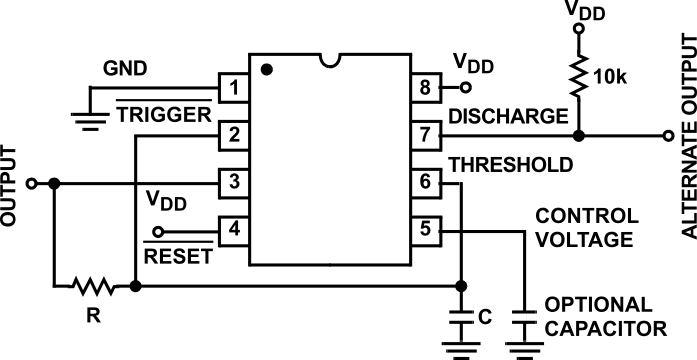
\includegraphics[width=0.75\linewidth]{Figures/6 PCB Design/555_astable.png}
\end{figure}

The two key components are the resistor \code{R} and the capacitor \code{C} whose respective resistance and capacitance control the output frequency \code{f} using the formula below \cite{icm7555}:

\[f = \frac{1}{1.4 R C}\]

\subsection{Creating Audio}
For this transmitter design, the 555 timer is used to create the precise frequency voltage changes needed to cause a speaker to play a specific tone.

- make the connection from one resistor to a switch alternating between four

- make the connection of attaching the speaker to the output line of the 555 timer.
\begin{figure}[h]
    \centering
    \caption{Centerpiece State Transmitter Circuit}
    \label{fig:555_astable_modded}
    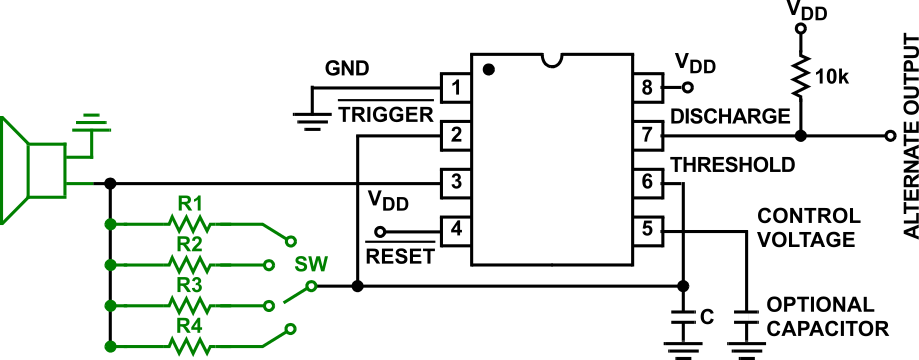
\includegraphics[width=\linewidth]{Figures/6 PCB Design/555_astable_modded.png}
\end{figure}

 - show the schematic (explain 555 timers -> connect to speaker -> add supporting components)

 - argue through the logic of the design (how it works to produce the desired tones)

\subsubsection{Choosing the values of \code{R} and \code{C}}
 - show the Excel chart figuring out which resistance/capacitance combos produce useful tones for the transmission.

TODO outline the process of choosing specific hardware to use for this project

\section{Prototyping}

TODO detail the process of building a prototype.

- Include pictures of the board and ...

- ... the generated spectrograms.

\section{Miniaturization}
- highlight the value of so few components for the physical size requirement, e.g. the prospects of A SMD version of the board

- Give a final part count.

- Talk about sizes for the components of the pcb.

- Discuss SMD versions

- If possible, create a demo in KiCAD...

\section{Minimizing Sound Obstruction}
TODO Discuss the "tupperware" tests -> design of various center caps.

\section{Summary}
